\section{PRAIS-WINSTEN ESTIMATION}
\label{sec:regression}
As we imagine there is a correlation between Interest Rate, Inflation and Gross Domestic Product, then we could ask: is there a way to model how changes in the first two variables affect the third, and can we predict how a country could change from a situation to another? We try to answer these questions in the following sections.

\subsection*{Statistical Background}
Ordinary Least Squares(OLS) is a widely used method for estimating the parameters of a linear regression model. However, OLS has some limitations, such as the assumption of homoscedasticity and the independence of the residuals. When these assumptions are violated, the estimates are biased and the standard errors are not reliable. Time series data often violates these assumptions, as the observation are not independent and the residuals are autocorrelated. There are several methods to deal with these issues, both with models specific for time series such as ARIMA models and with models that try to fix the data before applying OLS. One of these models is the Prais-Winsten Estimator \cite{prais}, which is a method to correct the OLS estimates by assuming the residuals are autocorrelated.

Consider the linear regression model
\begin{align*}
  y_t = \alpha + \beta x_t + \epsilon_t
\end{align*}
where we assume the residuals $\epsilon_t$ can be modelled as a first order autoregressive process $AR(1)$ $\epsilon_t = \rho \epsilon_{t-1} + e_t, |\rho|<1$. The Prais-Winsten Estimator is then obtained by applying the following transformation to the data:
\begin{align*}
  y_{t}-\rho y_{t-1}         & =\alpha (1-\rho )+(X_{t}-\rho X_{t-1})\beta + e_{t}                                                               \\\\
  {\sqrt {1-\rho ^{2}}}y_{1} & =\alpha {\sqrt {1-\rho ^{2}}}+\left({\sqrt {1-\rho ^{2}}}X_{1}\right)\beta +{\sqrt {1-\rho ^{2}}}\varepsilon _{1}
\end{align*}
This method is a modification of the Cochrane-Orcutt method \cite{cochrane}, but has the additional transformation for the first observation $y_1$ while the Cochrane-Orcutt method only transforms the data for $t>1$.

The Prais-Winsten Estimator is an iterative method, where we first estimate $\rho$ using the residuals of the OLS model and then apply the transformation to the data described above and fit a new OLS model until convergence. The convergence criteria can be based on the change in the estimates of $\rho$ or by statistical tests on the residuals such as the Ljung-Box test or the Durbin-Watson test.

Here we show the results of the Prais-Winsten Estimator on the data for Italy. As an introductory step, we show the time series for GDP, IR and CPI for Italy (Figure \ref{fig:italy_ts}).
\begin{figure}[H]
  \includegraphics[width=.9\linewidth]{imgs/italy_gdp.png}
  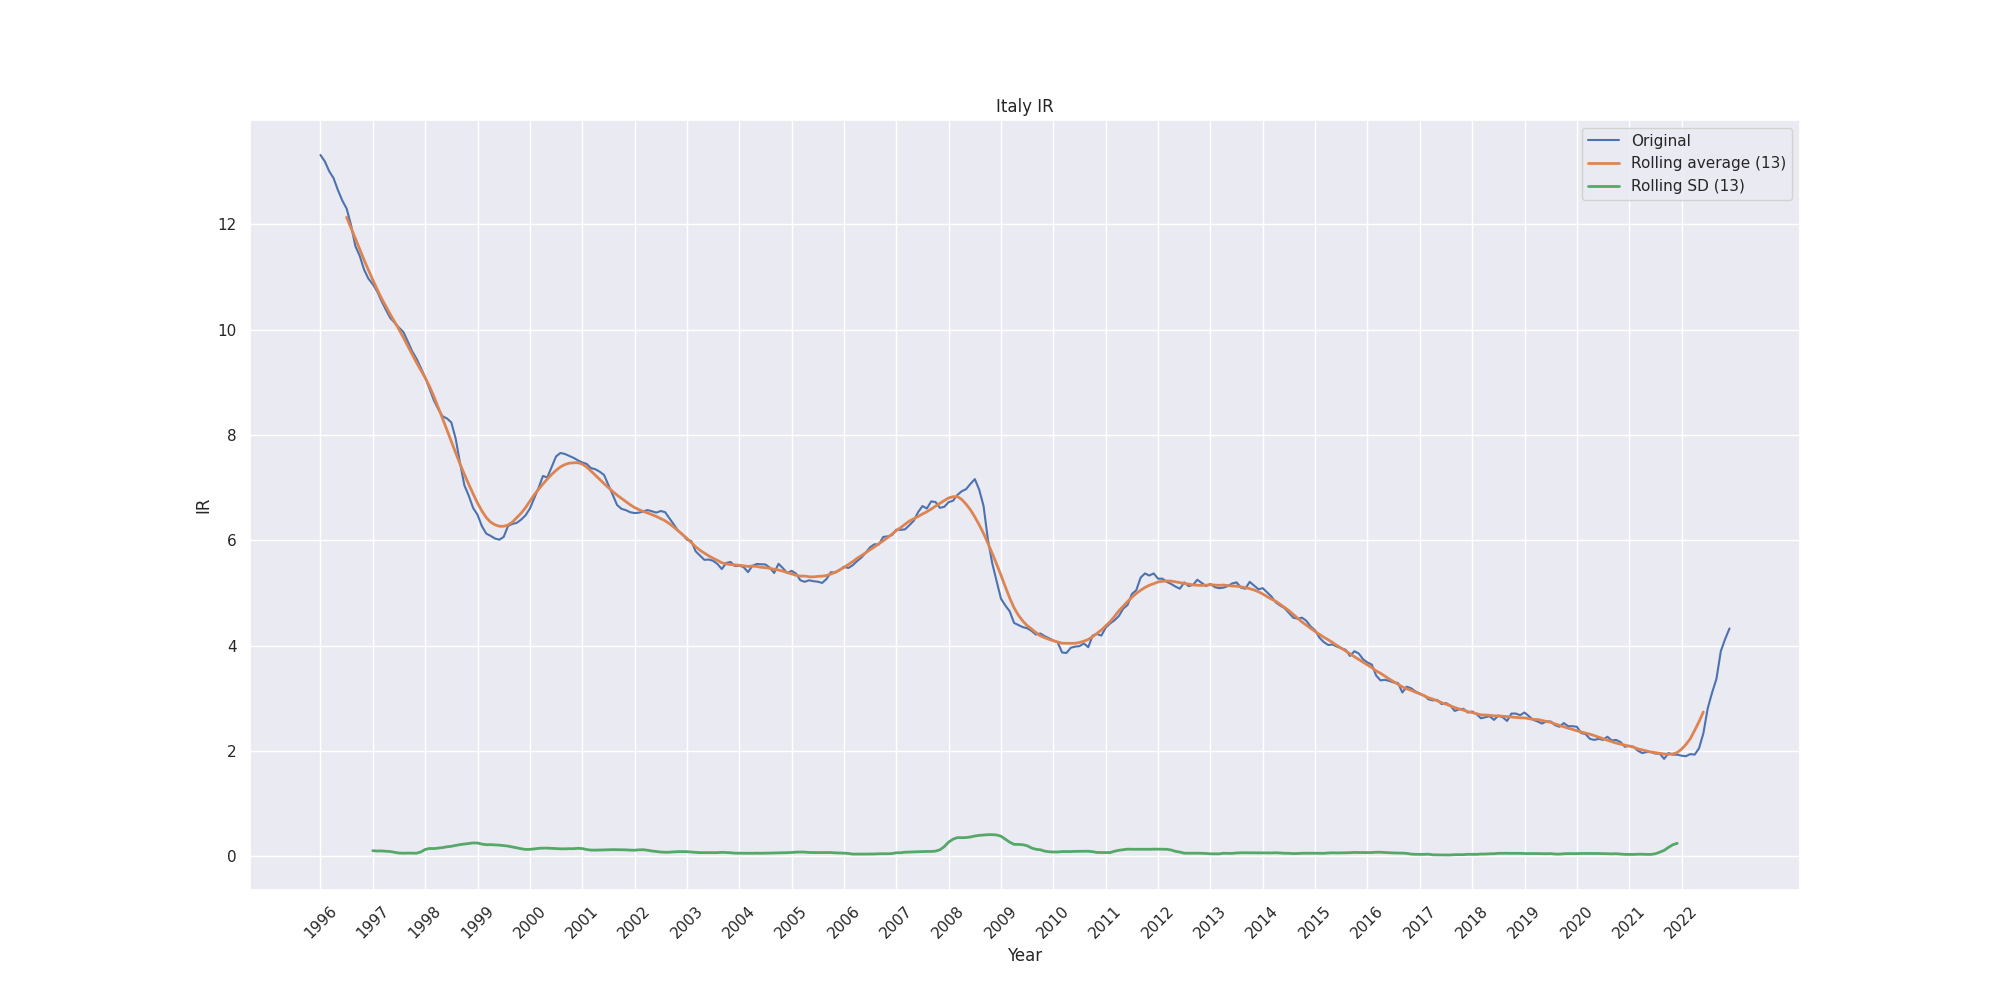
\includegraphics[width=.9\linewidth]{imgs/italy_ir.png}
  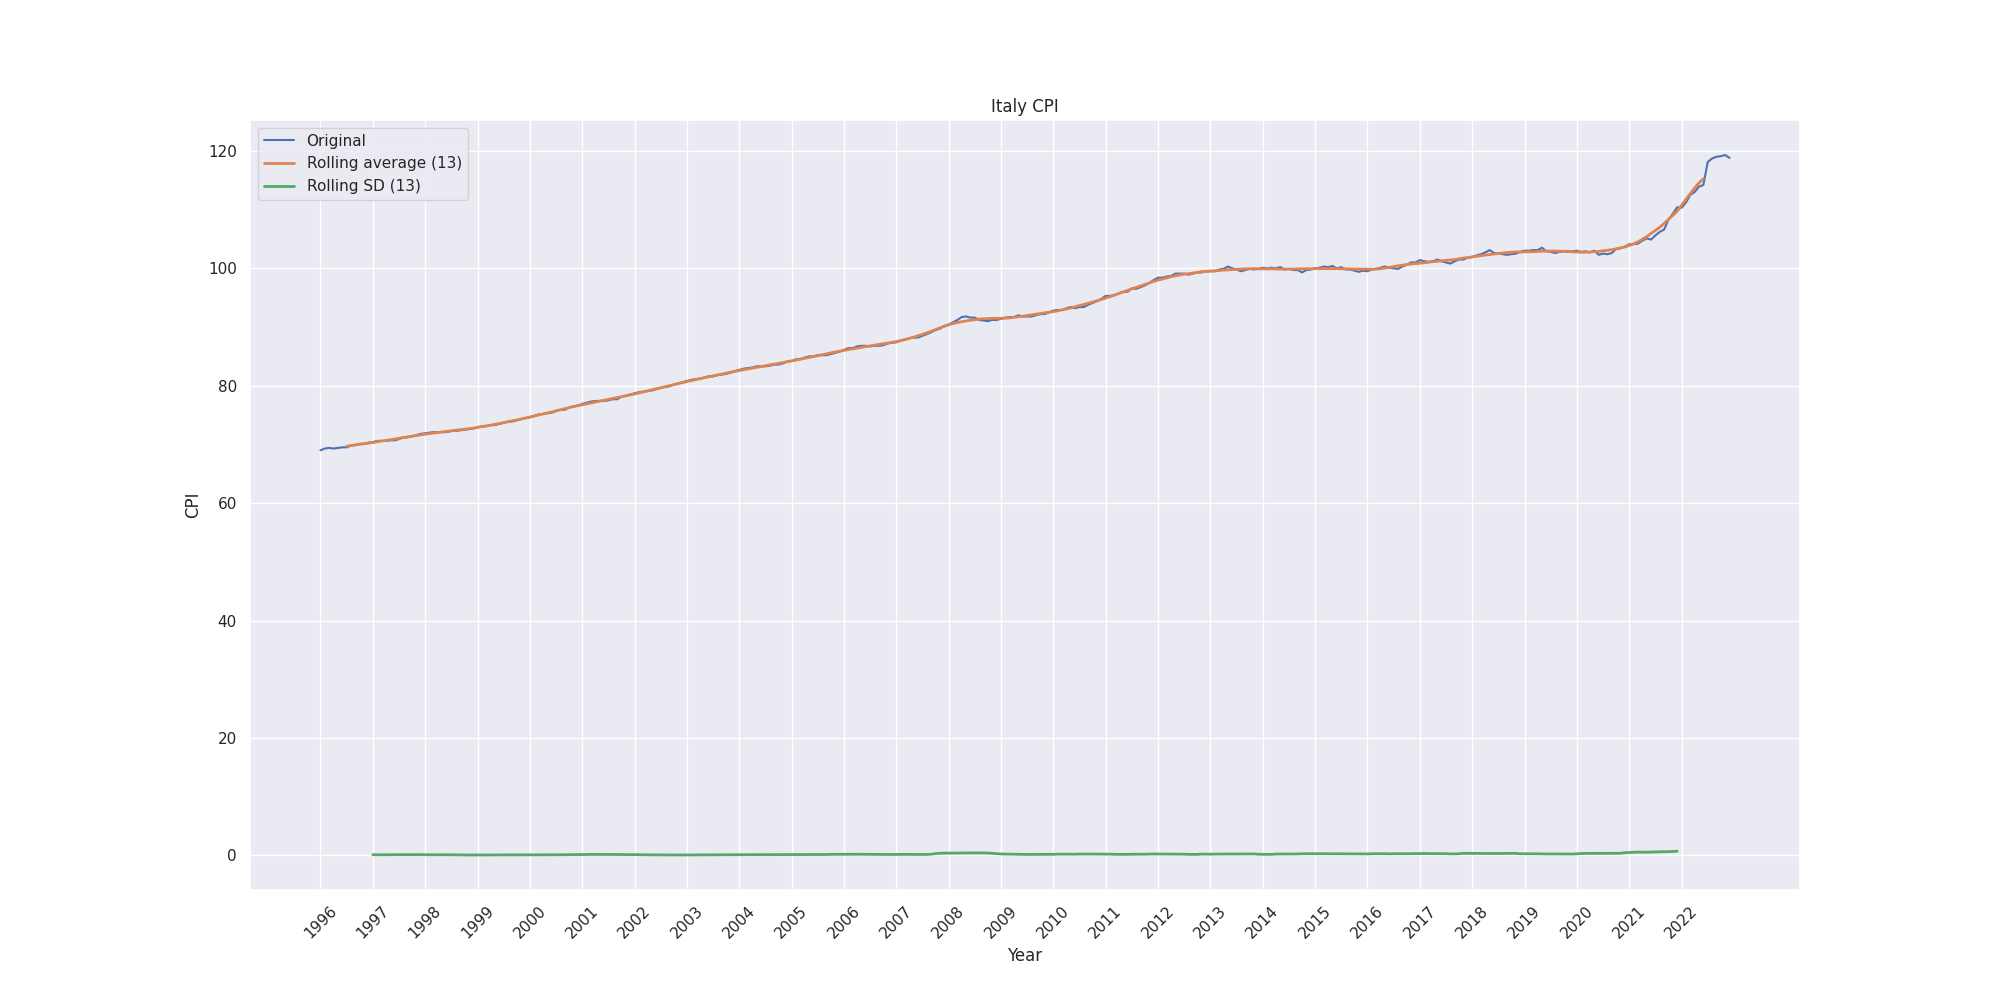
\includegraphics[width=.9\linewidth]{imgs/italy_cpi.png}
  \caption{Time series for Italy}
  \label{fig:italy_ts}
\end{figure}


We can see that the time series for GDP, IR and CPI are not stationary, so we first take the first differences (Figure \ref{fig:italy_diff}) which means we subtract the value at time $t-1$ from the value at time $t$. This transformation allows us to make data stationary and reduce autocorrelation.

\begin{figure}[H]
  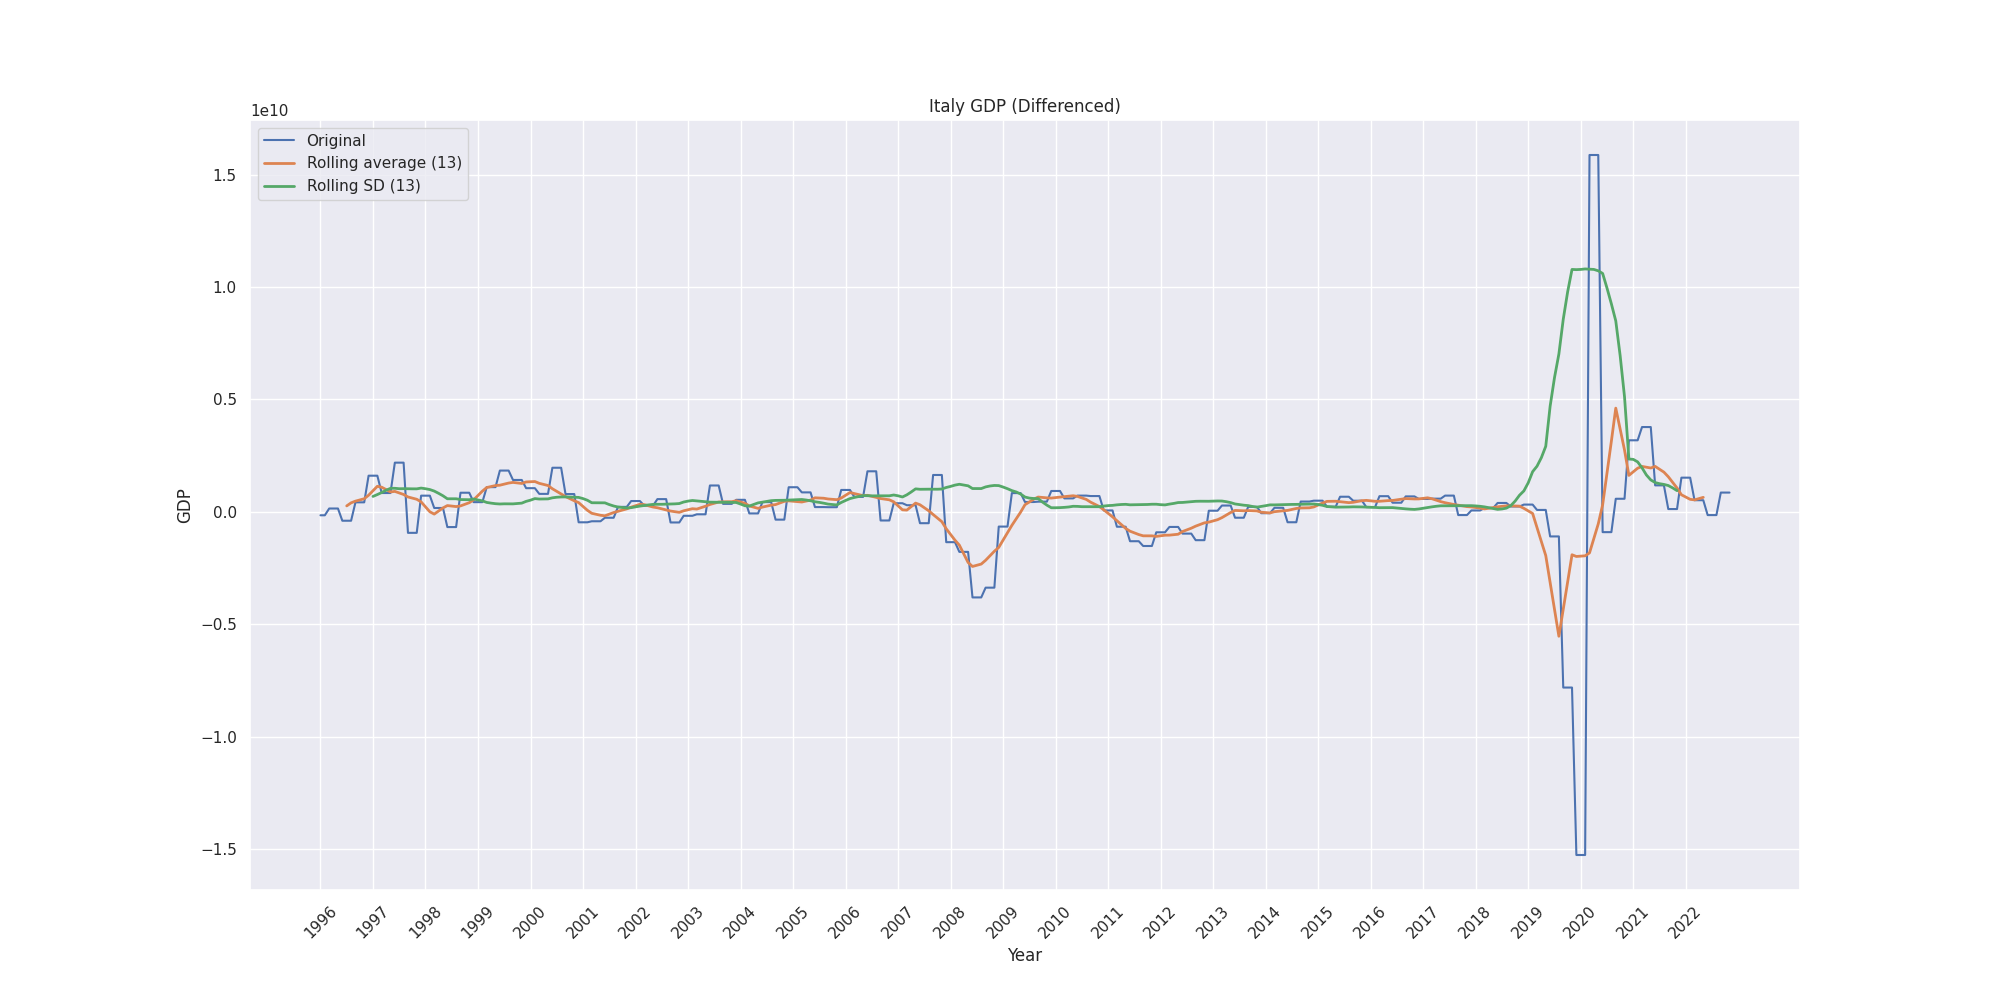
\includegraphics[width=.9\linewidth]{imgs/italy_gdp_diff.png}
  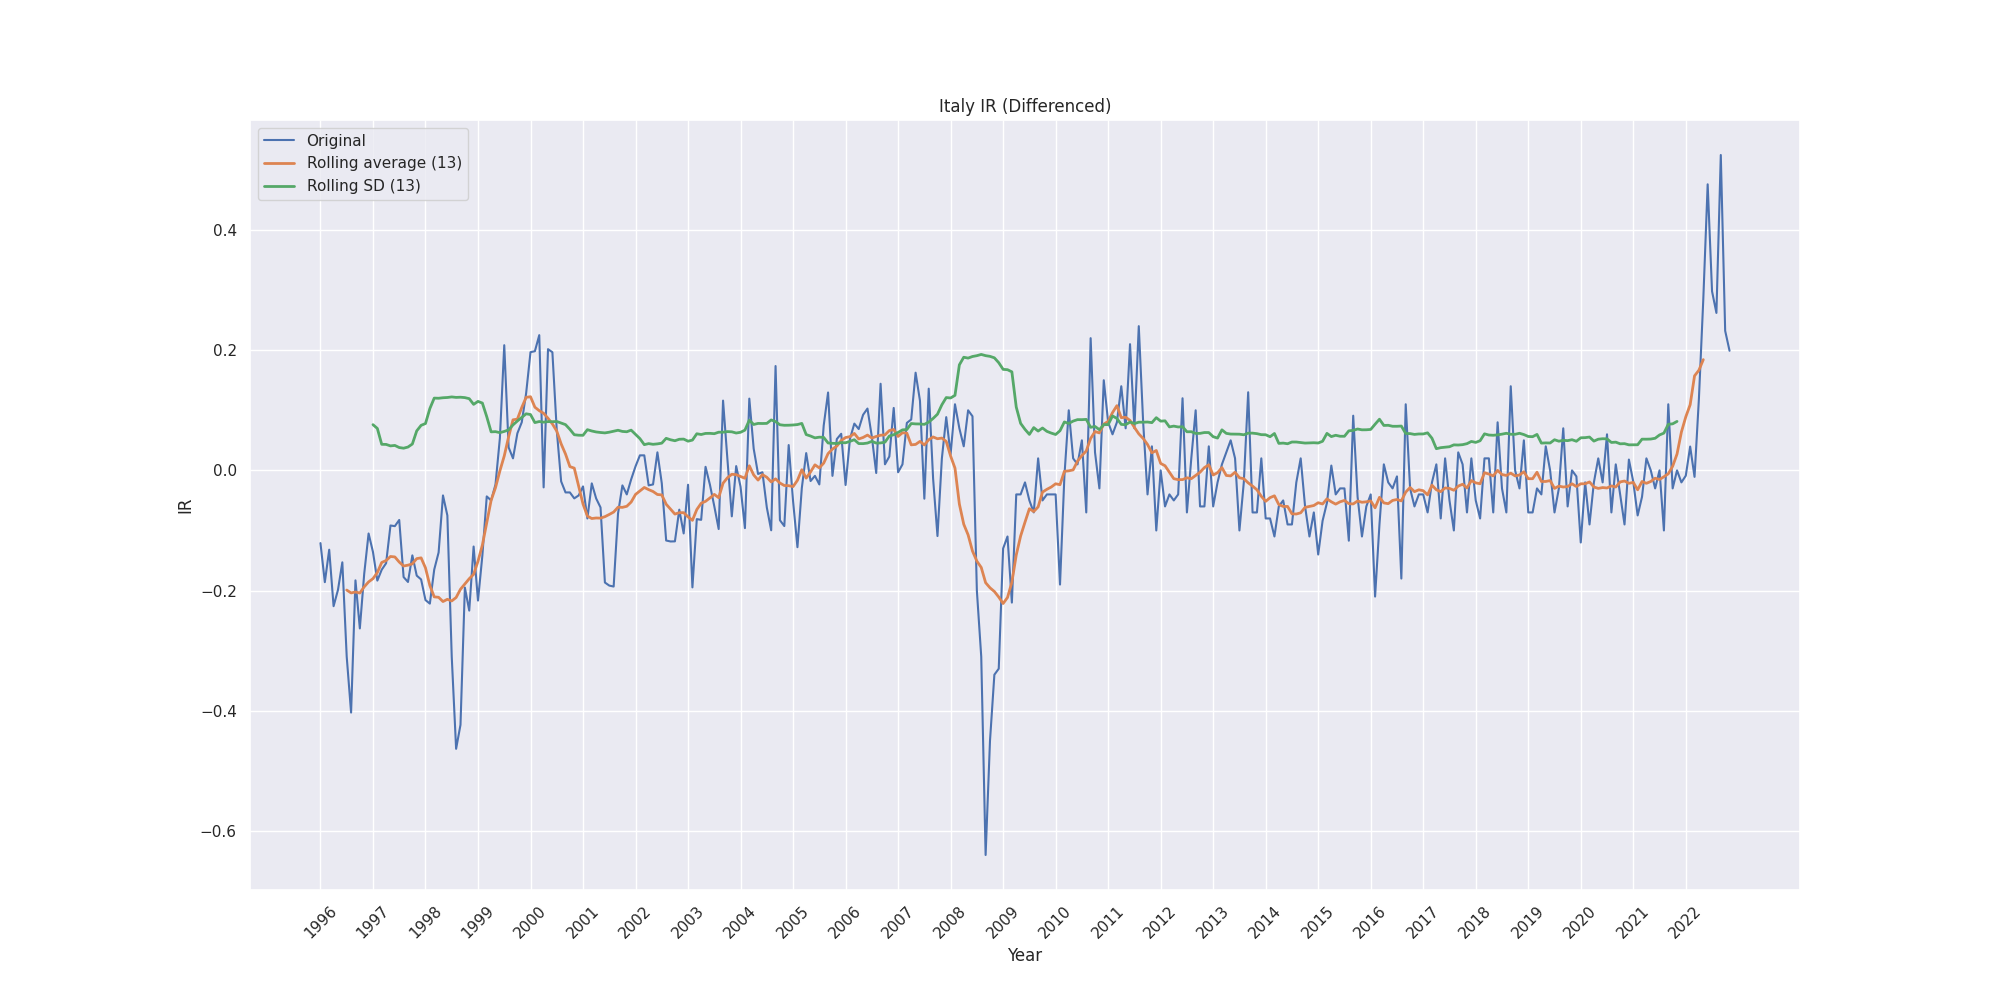
\includegraphics[width=.9\linewidth]{imgs/italy_ir_diff.png}
  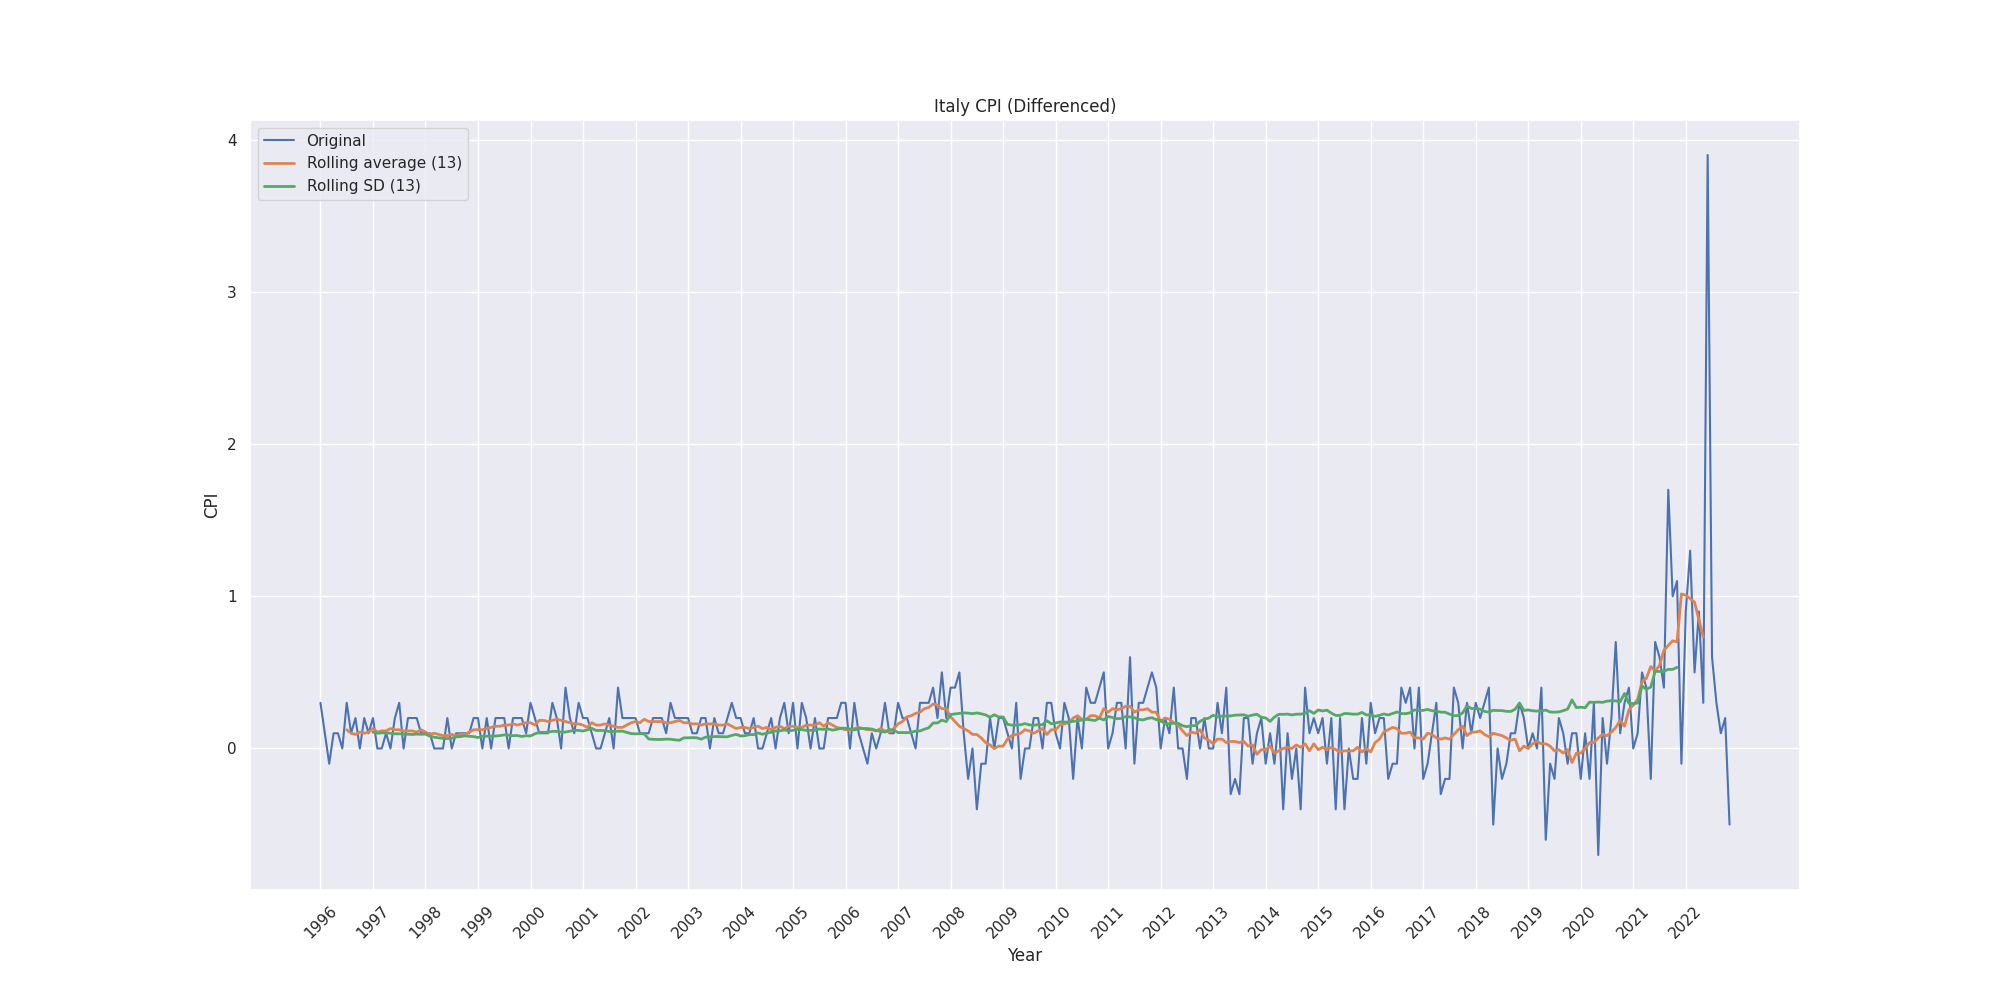
\includegraphics[width=.9\linewidth]{imgs/italy_cpi_diff.png}
  \caption{Time series first differences for Italy}
  \label{fig:italy_diff}
\end{figure}

The algorithm is shown in the following pseudo-code:
\begin{lstlisting}[language=Python]
def fit(x,y):
  model = OLS(y,x).fit()
  rho = compute_rho(model)
  while not convergence_criteria:
      model = prais_winsten(model, rho)
      rho = compute_rho(model)
  return model, rho

def compute_rho(model):
  e_0 = model.resid[1:]
  e_1 = model.resid[:-1]
  return np.dot(e_1,e_0)/np.dot(e_1,e_1)

def prais_winsten(self, model, rho):
  x_0 = np.sqrt(1 - rho**2) * x[0]
  y_0 = np.sqrt(1 - rho**2) * y[0]
  x_t = x[1:,] - rho * x[:-1,]
  y_t= y[1:] - rho * y[:-1]
  x = np.append(x_0, x_t, axis=0)
  y = np.append(y_0, y_t)
  return OLS(y, x).fit()
\end{lstlisting}

\subsection*{Results}
We then apply the Prais-Winsten Estimator to the differenced data. The results of the regression are shown in Table \ref{tab:italy_pw}. As we can see the results are inconclusive, as the R-squared is very low and the p-value is only significant for the Interest Rate variable. Moreover the coefficients are very close to zero, which probably implies that the model is not a good fit for the data.

\begin{center}
    {\small
  \begin{tabular}{cccccc}
                             & \textbf{coef} & \textbf{std err} & \textbf{t} & \textbf{P$> |$t$|$} & \textbf{[0.025 0.975]} \\
    \hline    \textbf{const} & 0.0009        & 0.009            & 0.096      & 0.924               & [-0.017 0.019 ]        \\
    \textbf{ir}              & -0.0080       & 0.003            & -2.561     & 0.011               & [-0.014 -0.002]        \\
    \textbf{cpi}             & -0.0020       & 0.001            & -1.659     & 0.098               & [-0.004 0.000 ]        \\
    \hline
  \end{tabular}
  }
  \begin{tabular}{lc}
    Statistics                              &        \\
    \hline
    \textbf{  R-squared (uncentered):}      & 0.042  \\
    \textbf{  Adj. R-squared (uncentered):} & 0.031  \\
    \textbf{  F-statistic:       }          & 3.605  \\
    \textbf{  Prob (F-statistic):}          & 0.0141 \\
    \textbf{  Log-Likelihood:    }          & 900.71 \\
    \textbf{  AIC:               }          & -1795. \\
    \textbf{  BIC:               }          & -1785. \\
    \textbf{No. Observations:}              & 248    \\
    \textbf{Df Residuals:}                  & 245    \\
    \hline
  \end{tabular}
  \label{tab:italy_pw}
\end{center}


In the regression's diagnostic plots in Figure \ref{fig:italy_diag} we can see in the residuals vs fitted plot that the residuals can be considered white noise and the QQ plot is acceptable to suggest normality. However, even if all these plots don't seem to show any major issue, the low R-squared and the non-significant p-values suggest that the model is not a good fit for the data anyway.
\begin{figure}[H]
  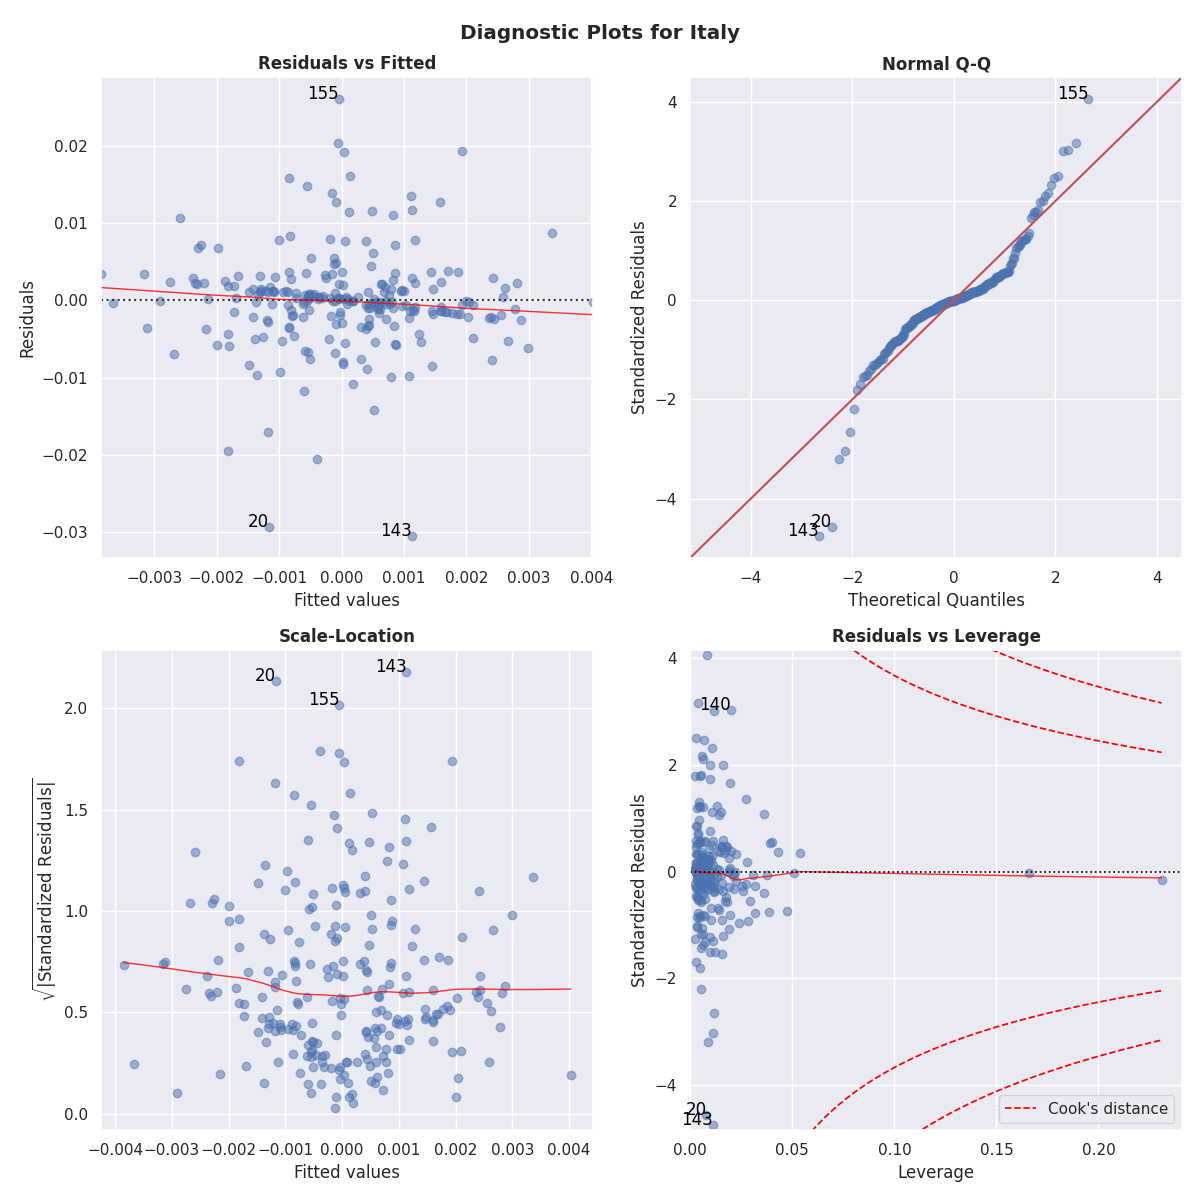
\includegraphics[width=.9\linewidth]{imgs/italy_diagnostic_plots.png}
  \caption{Diagnostic plots for Italy}
  \label{fig:italy_diag}
\end{figure}

This lack of fit can be further confirmed by predicting the future values of GDP using the model both for the test set and for the COVID data. We can see that the prediction is roughly constant but more importantly the prediction intervals are extremely wide, which means that the model is not able to predict the future values of GDP with any degree of certainty (Figure \ref{fig:italy_pw_pred}).
The prediction intervals are computed according to this paper \cite{prais_ci}
\begin{align*}
  \hat{Y_t} \pm t_{1-\alpha/2, n-2} \eta_n
  \eta_n = \hat{\sigma} \left( \frac{\sum_{i=1}^n(X_i - X_t)^2}{n \sum_{i=1}^n (X_i - \bar{X})} + \frac{1}{1-\hat{\rho}^2} \right)
\end{align*}

Moreover, it is interesting to note the chart of the one-step ahead predictions, which uses the true values of GDP up to time step $t-1$ to predict exclusively the value at time step $t$. This graph is satisfactory, as the predictions are very close to the true values, but the task is much simpler since only one step is predicted.
\begin{figure}[H]
  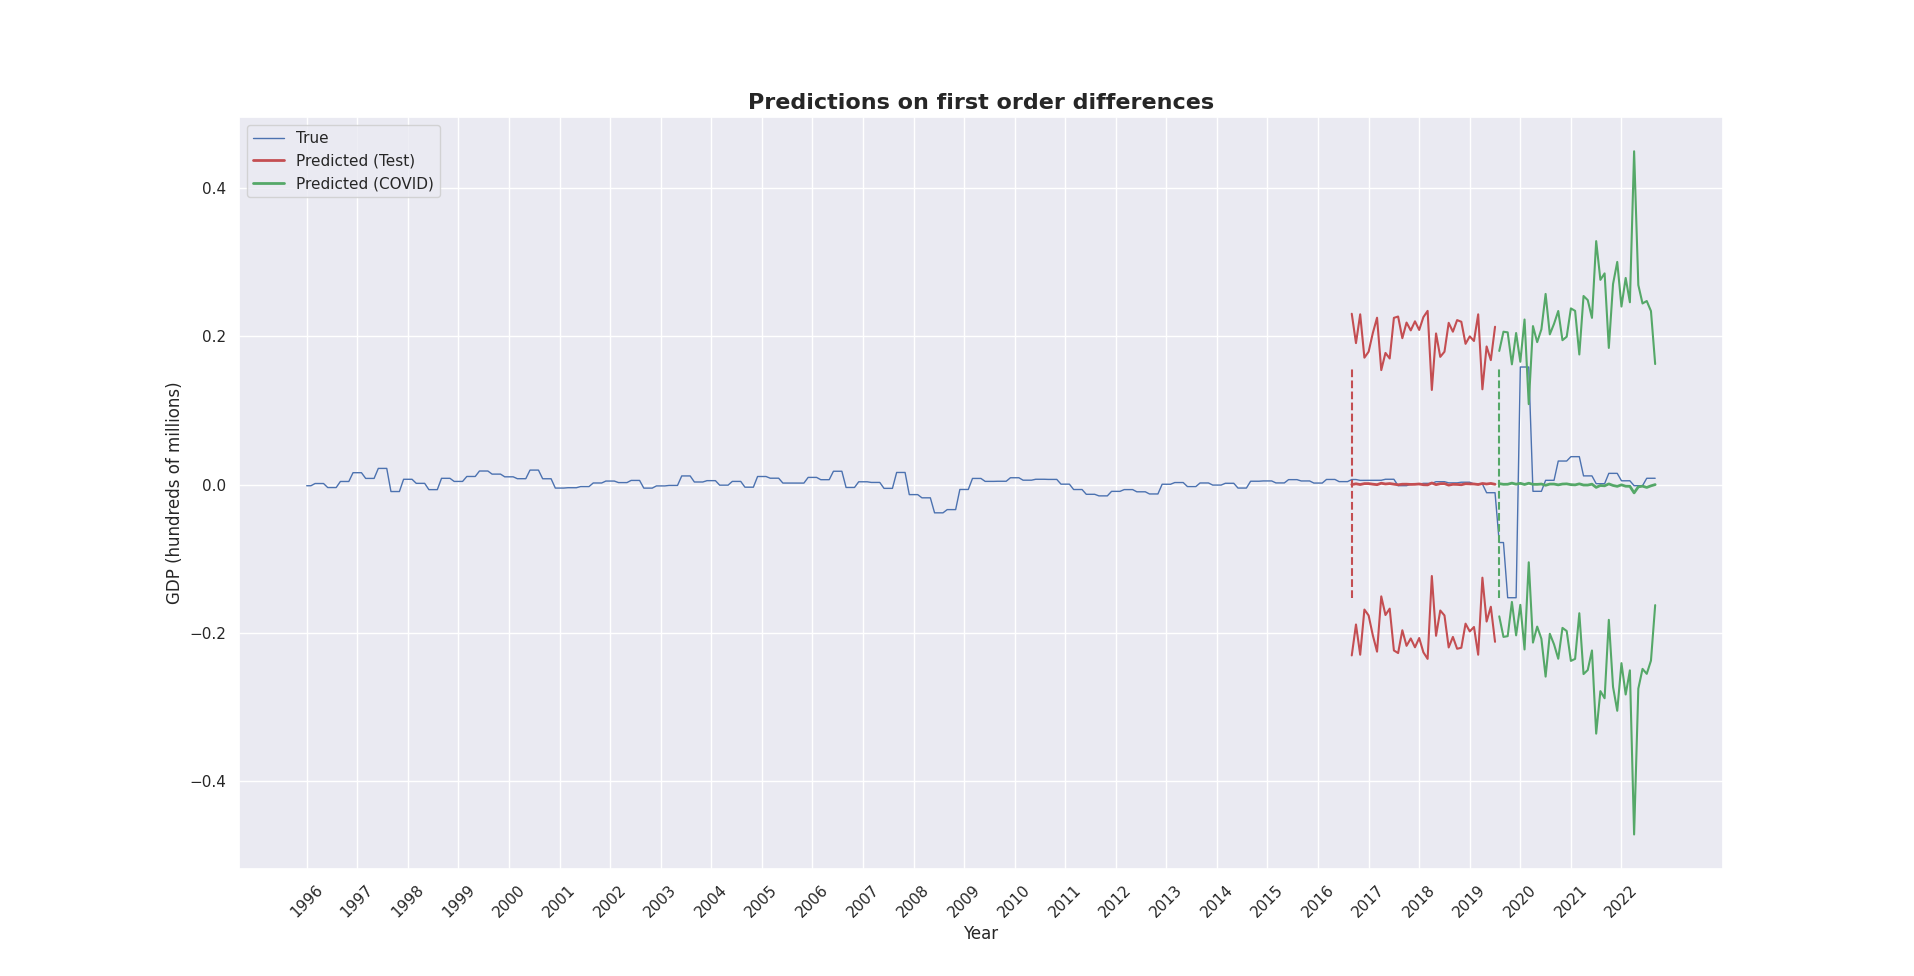
\includegraphics[width=.9\linewidth]{imgs/italy_pred_diff.png}
  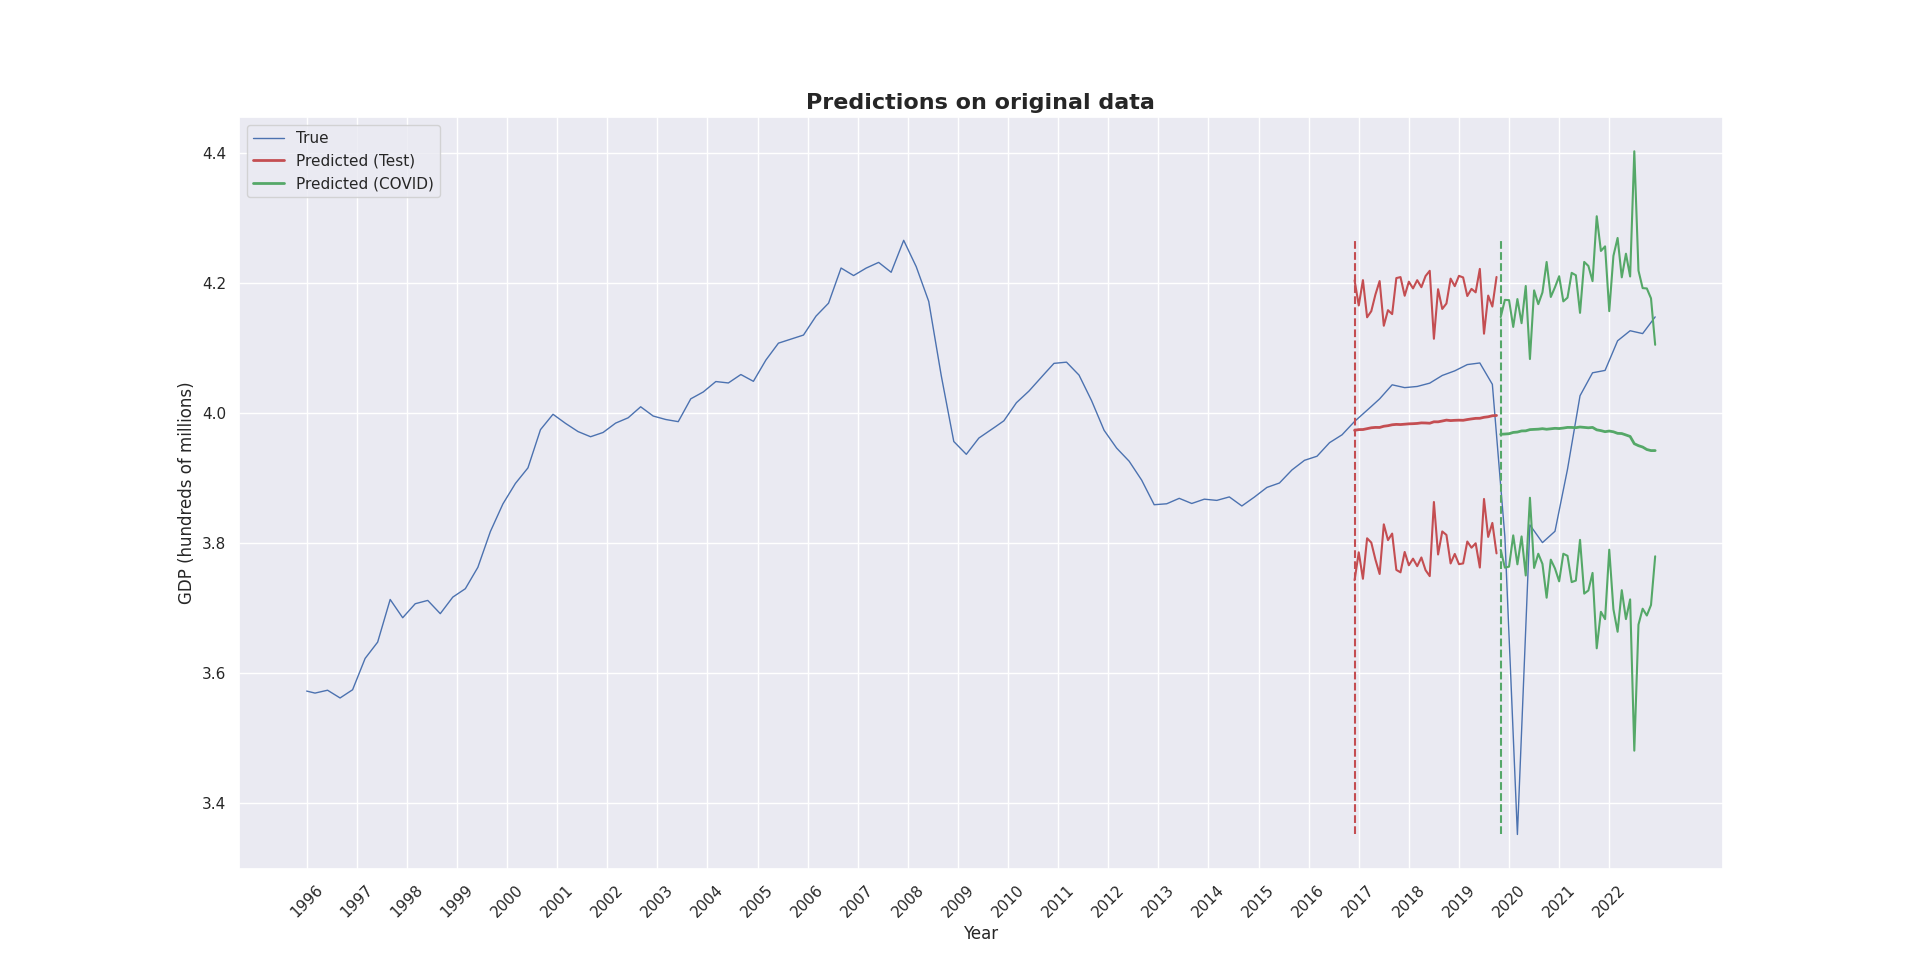
\includegraphics[width=.9\linewidth]{imgs/italy_reg_predictions.png}
  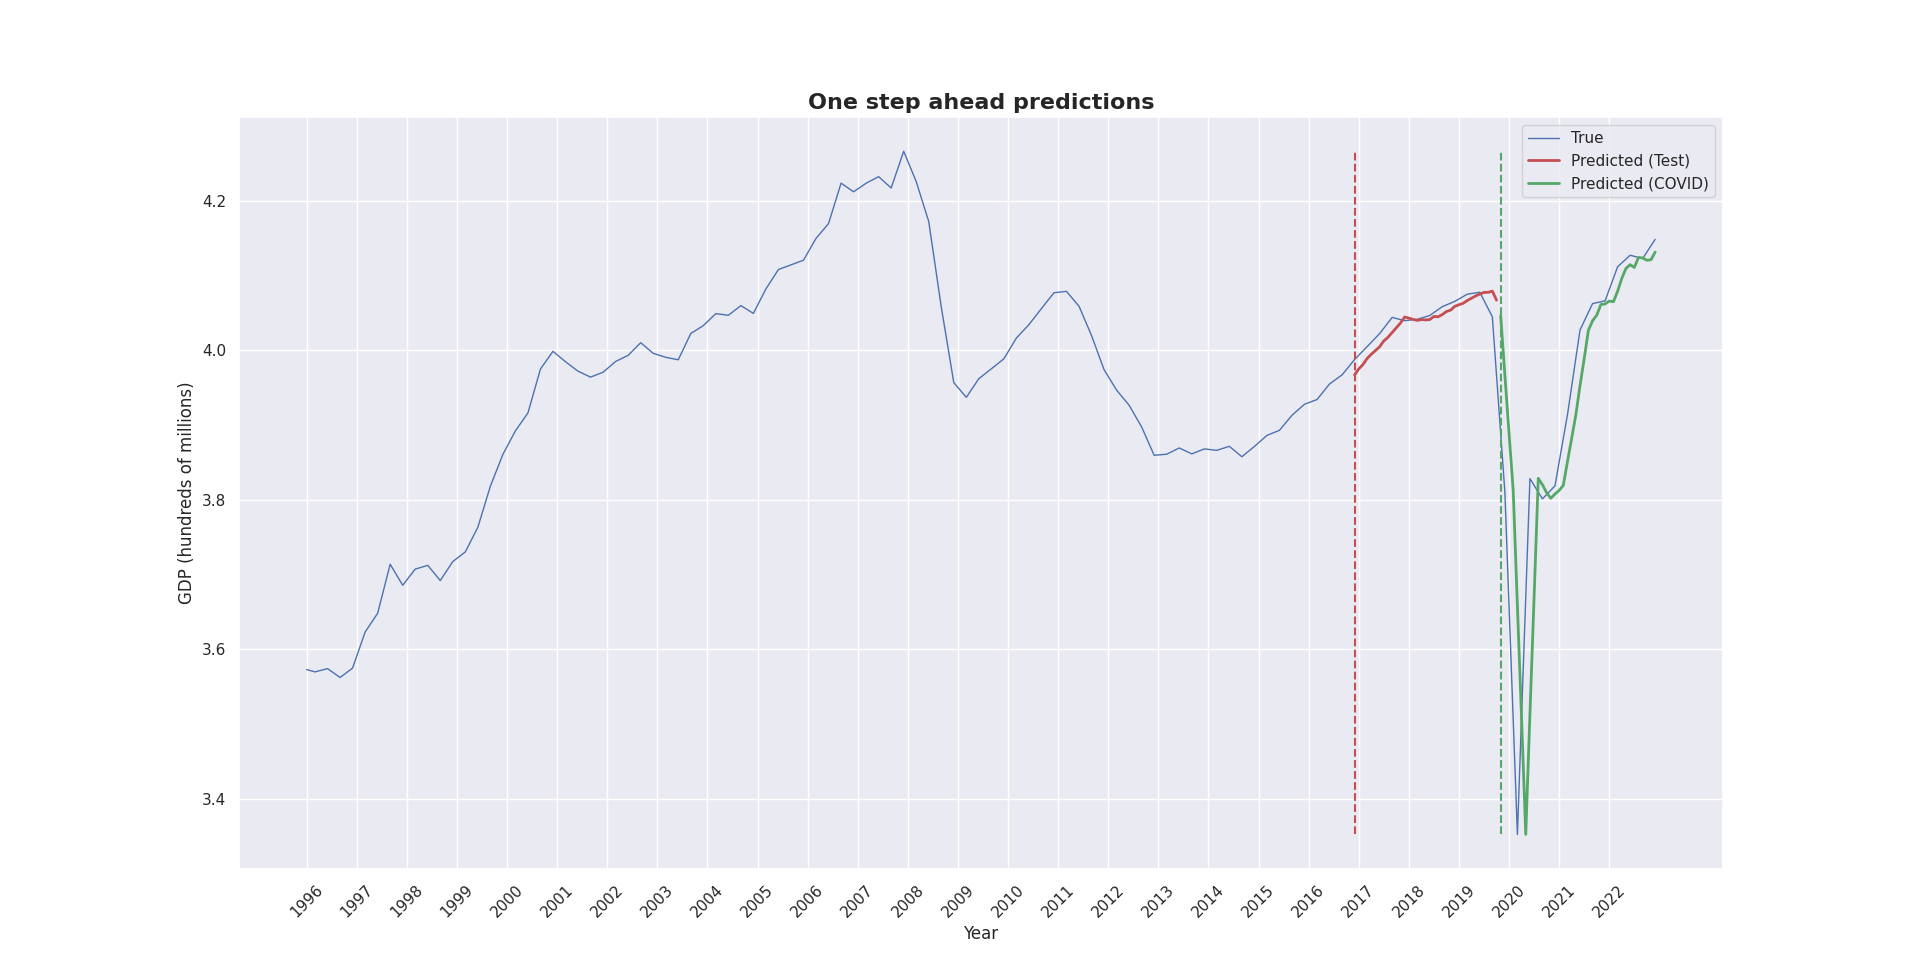
\includegraphics[width=.9\linewidth]{imgs/italy_pred_one_ahead.png}
  \caption{Prais-Winsten Estimator predictions for Italy}
  \label{fig:italy_pw_pred}
\end{figure}

The most probable reason for the poor performance of the model is that the assumption that the residuals are modelled by an $AR(1)$ process is very simplistic and does not capture the complexity of the data. By observing the ACF and PACF of the residuals (Figure \ref{fig:italy_res_corr}) we can see that the residuals are not well modelled by an $AR(1)$ process, as there are several lags that are significant and the ACF does not decay quickly. This implies that the residuals are not white noise and the model is not a good fit for the data. A possible improvement that could be done is to try a more complex model for the residuals; given that both the autocorrelation and the partial autocorrelation exhibit a sinusoidal pattern an ARMA model could be considered \cite{ts_intro}pg.356.
\begin{figure}[H]
  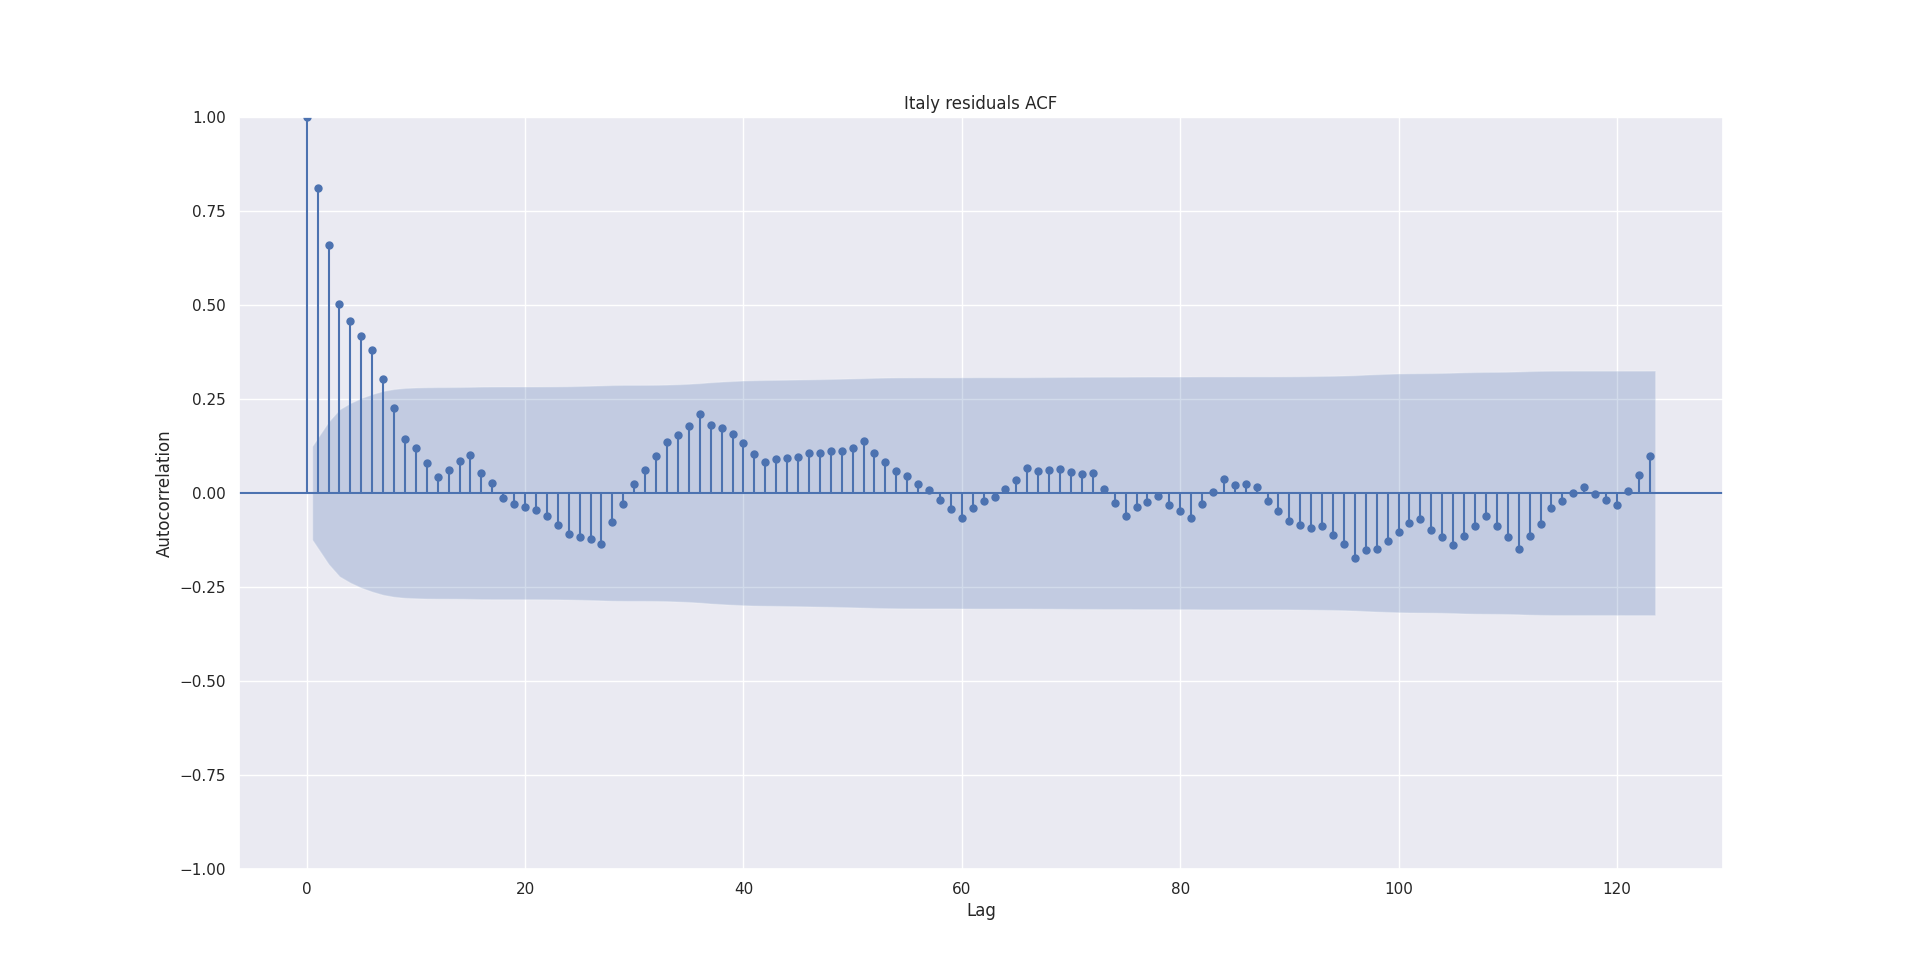
\includegraphics[width=.9\linewidth]{imgs/italy_res_acf.png}
  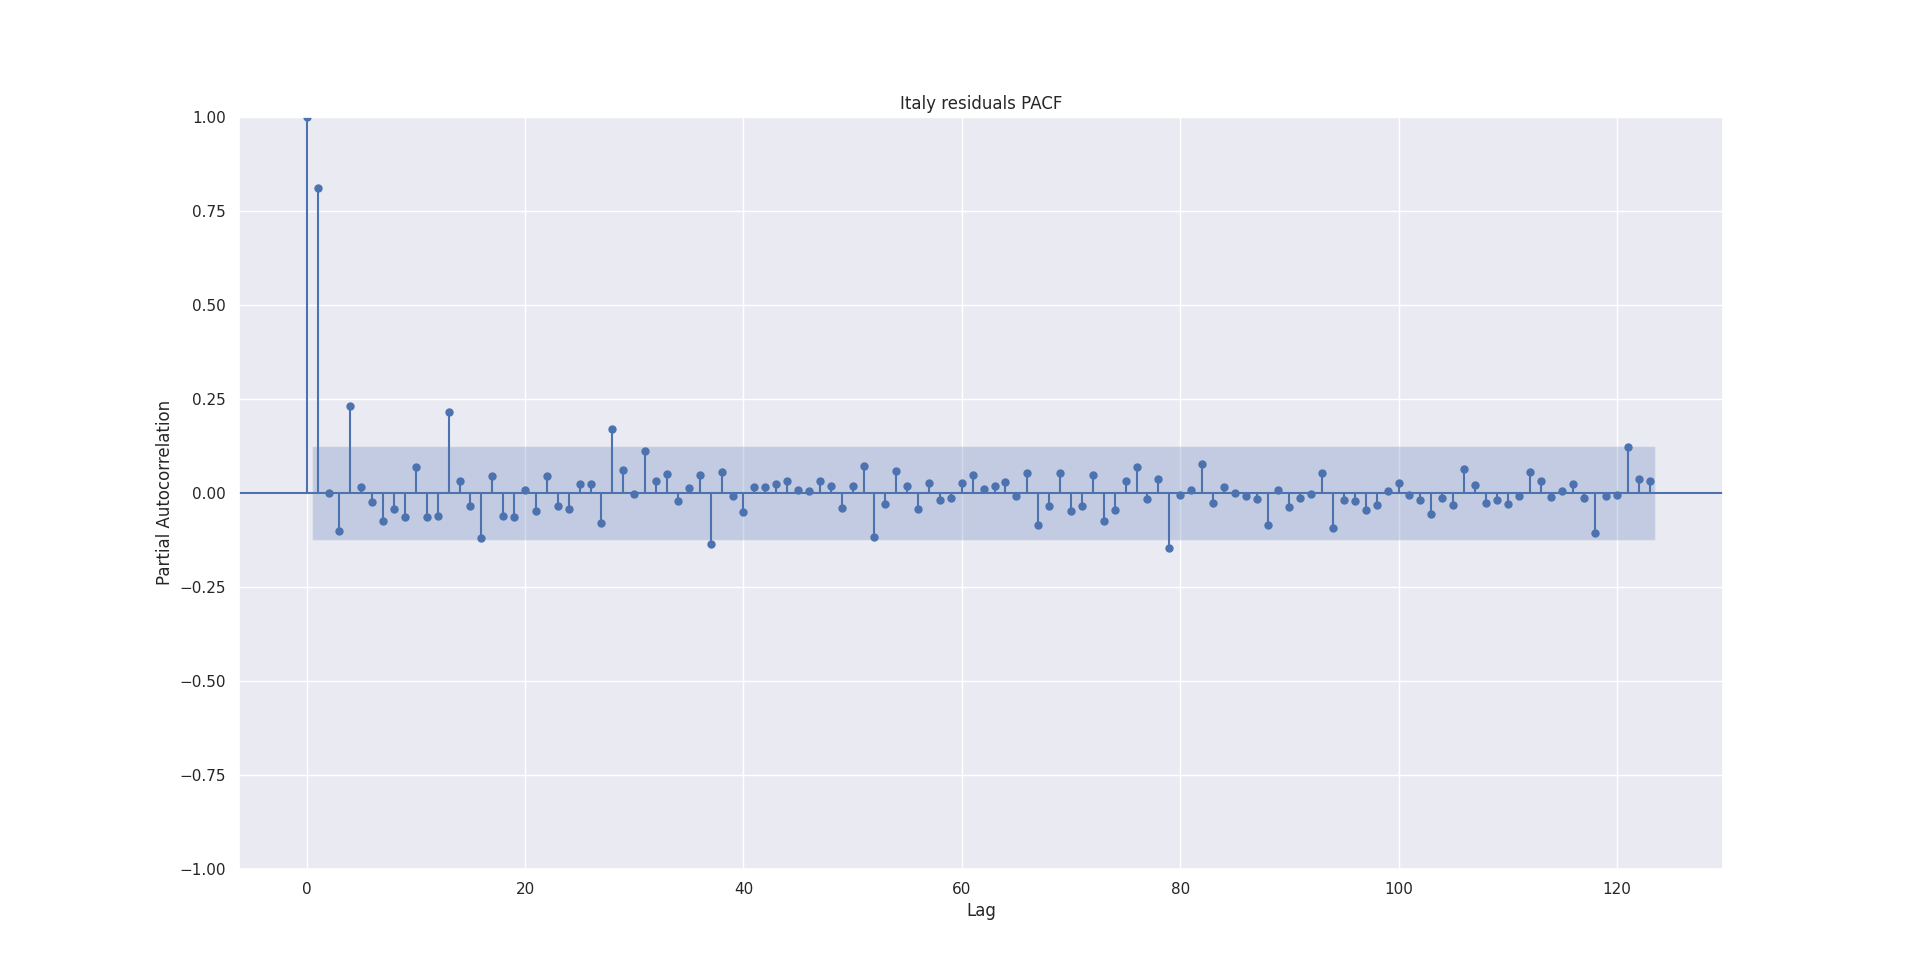
\includegraphics[width=.9\linewidth]{imgs/italy_res_pacf.png}
  \caption{Residuals ACF and PACF for Italy}
  \label{fig:italy_res_corr}
\end{figure}

Another, more straightforward, improvement could be to include more variables in the regression, as the model is extremely limited with only two variables.
